\chapter{The Quest for a Quantum Computer}
Before delving into the question of how we might build a quantum computer, it is worth taking a step
back and exploring the question of what brought us as a scientific community to the point where
it is seen as a priority to build one. The answer to that requires us to delve briefly into
the world of computational complexity theory, and to examine what it means to solve problems "efficiently".
Although the genesis of computation can be traced back to pioneering works by people such as Charles Babbage
and Ada Lovelace in the early 1800's~\cite{Bowden:1953:FTS:1102044}, it was not until the early 1900's that
machines we might recognize as computers were constructed. Based on delicate vacuum tubes, mechanical relays
and often taking up full rooms, their inherent fragility and bugginess posed formidable obstacles to scaling. 
It was not until the mid 1900's that the field really took off with two key discoveries. The first
was the construction of the first transistor in 1947, credited to Bardeen, Brittain and Schockley and for which
they were awarded the Nobel prize in 1956~\cite{nobel1956}. This was followed by the creation of integrated circuits by Jack Kilby
in 1959, for which he was awarded the Nobel prize in the year 2000~\cite{nobel2000}. With these two inventions, a remarkable 
surge in computational power occured. This surge is embodied in 'Moore's law', which described an annual
doubling in the number of transistors that it would be possible to fit on a single integrated circuit~\cite{4785860}.
And with this doubling came an exponential growth in the computation power that we had available to us.

Along with this growth came an obvious question. What exactly can these computers do? What sorts of
problems will we be able to solve with our ever growing bundle of transistors? To do this, we need to
think about how many steps it takes to run various algorithms. Take for example the question of looking
for a single item $x_T$, in a list $L = \{x_0, x_1, ..., x_n\}$ with $n$ items in it. Assuming the list
is in an unknown order, to find the location of the item $x_T$, we need to look at each item in the list
in turn. If the length of the list were doubled to $2n$ items, it would take twice as many comparisons to
look through the list. Tripled would be three times. The amount of time it takes to find an item in the
list is \emph{linear} in the length of the list. We can write this mathematically using big$\mathcal{O}$ 
notation: searching for an item in a list is $\mathcal{O}(n)$. 

What about a slightly more complicated problem. What if we want to check whether any item $x_i$ appears
in the list twice? To run this algorithm, we can run the above algorithm for each item in the list, setting the
target to $x_T = x_0$, then $x_T = x_1$ and so forth, and checking whether we find the item two or more
times. So for $n$ items in the list, we run through the list $n$ times, so the number of steps to run
the algorithm scales as $\mathcal{O}(n^2)$. That is, if the length of the list is doubled, it takes
four times as long, so the scaling is \emph{quadratic}.
In this way we can classify algorithms into various complexity classes. For example, sorting a list
of $n$ items is in the best case $\mathcal{O}(n \log(n))$. Solving the travelling salesman problem (TSP) is
$\mathcal{O}(n^2*2^n)$. More generally, we can group problems into those that have at worst a polynomial
complexity, i.e. $\mathcal{O}\left(f(n)\right)$ where $f(n)$ is a polynomial. These problems are are
in the complexity class \cc{P} (for polynomial), and are said to be \textbf{efficiently} computable.
Those problems that have a difficulty that grows faster than a polynomial in the size of the problem, 
for example problems whose complexity grows exponentially, are said to be inefficcient to compute.

Of course, you might say, well what sort of operations do we allow our computers to do in a single step?
If I say that my computer can solve the TSP in a single step, then the complexity reduces trivially to
$\mathcal{O}(1)$. The answer is not so trivial --- it is limited by the laws of physics. What sorts
of computation do they allow? To answer this question, Alan Turing and Alonzo Church came up with the notion of 
the Turing Machine, a universal model for a computational device, and with it stated the Church-Turing 
hypothesis:

\begin{displayquote}[\cite{turingthesis}]
  "a function is effectively calculable if its values can be found by some purely mechanical process". 
  We may take this literally, understanding that by a purely mechanical process one which could be carried out by a machine.
\end{displayquote}

To paraphrase, this stated that anything a Turing machine could do, a computer could do too, and anything
it \emph{can't} do, no computer can. It wasn't long before this was extended to the strong Church-Turing
hypothesis, which states \textquote[\cite{kaye2007an}]{A probabilistic Turing machine can efficiently simulate any 
realistic model of computation}.
\footnote{In fact, we have to make an addition to the class of algorithms that our Turing machine can run efficiently,
 due to the discovery of probabilistic algorithms, which can solve some problems with $> 2/3$ chance in
 poynomial time. By running these algorithms repeatedly we can solve problems to within an arbitrarily small 
 error $\epsilon$. This class of efficiently computable functions is called bounded-error probabilistic polynomial (\cc{BPP}).}
Note the addition of the \textbf{efficiently}, which means that for any
operation we could add to any hypothetical computer, we can get at most a polynomial speedup. Since
a polynomial $P(n)$ divided by another polynomial $Q(n)$ is a polynomial, and anything that grows faster
than a polynomial $E(n)$ divided by a polynomial $Q(n)$ still grows faster than a polynomial, we have
have a universal definition for problems that are efficient to solve and those that aren't.
\footnote{Of course, since we're constantly coming up with better algorithms to solve hard problems,
the set of problems that are efficient to solve seems to keep growing!}


\begin{figure}
  \includegraphics[width=0.7\linewidth]{MooresLaw}
  \caption[Moore's Law and the end of exponential scaling]
  {Graph of the number of transistors per chip, their clock speed, and their
  thermal design power plotted on a log scale against time. Although the number of transistors per chip
  continues to grow exponentially, the clock speed and power per chip has plateaued in the early 2000s.
  Reproduced with permission from~\cite{cross_2016}.}
  \label{fig:mooreslaw}
\end{figure}

So we've established what sorts of problems a computer can solve efficiently, and we've also noted the
expoential growth in the number of transistors on chip. As long as both of these facts remain true, we
should only have to wait a few years before our computers became twice as powerful and problems that were
previously intractable fall within our grasp. But of course, any exponential scaling must eventually fail
and so it was for ICs for two key reasons: power and transistor size. As we made our transistors smaller,
we stopped seeing a concomitant efficiency increase, and all of a sudden, the power density of our ICs 
became a limiting factor. In order to halt this increase we had to reduce power dissipation, and the
only way we saw how was by capping the speed of our computers, which we can see in figure~\ref{fig:mooreslaw}
has plateaued since the early 2000s. And the smaller our transistors became, the more costly they became 
to make. Even Moore's law, which has stubbornly held past the expectations of most scientists, must eventually
end as we bump up against the sizes of atoms. It seems unlikely that there is much room below Samsung's 
recently announced \SI{3}{\nano\meter} node, so if we want to bring more problems into the fold of the
possible, it seems like the strong Church-Turing hypothesis must give.

It was in this context that Feynmann gave his seminal address, noting that as far as we can tell, simulating
quantum systems falls outside of the set of problems that are efficient on classical computers\cite{Feynman1982}. 
However, as long as we are able to manipulate quantum systems, we should also be able to set up a "quantum
simulator" to see how a quantum system behaves. If this turned out to be the case, then the strong 
Church-Turing hypothesis would be violated!\footnote{Despite this violation, as far as we know the original
Church-Turing hypothesis still holds. No previously uncomputable function became computable with the addition
of quantum physics.} Here was nature efficiently simulating a system that as far as we know a Turing machine 
can't. It was David Deutsch who in 1985 formalized the idea of a quantum Turing machine\cite{doi:10.1098/rspa.1985.0070}, 
and laid out the Deutsch-Church-Turing hypothesis, which as far as we know holds to this day:

\begin{displayquote}
  A quantum Turing machine can efficiently simulate any realistic model of computation.
\end{displayquote}

\begin{figure}
  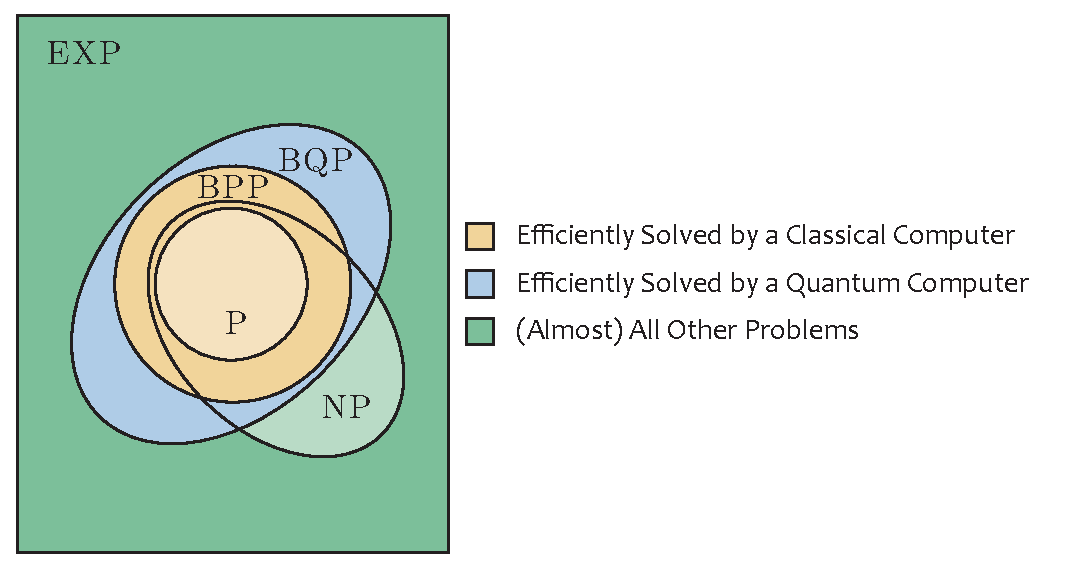
\includegraphics[width=0.85\linewidth]{ComplexityClasses}
  \caption[Relationship between various complexity classes]
  {Relationship between the various complexity classes that we've discussed. The class
  \cc{BPP} includes all problems that a classical computer can solve efficiently (including
  everything that can be calculated in polynomial time), \cc{BQP} is all problems a quantum computer can solve
  efficiently (which includes everything a classical computer can do). Finally, problems that scale exponentially
  with input size, labelled \cc{EXP}, is (almost) all other problems that are computable. The class
  \cc{NP} is also included on this figure as it is one that often comes up in the context of complexity,
  if for no other reason than to emphasize that a quantum computer \emph{cannot} solve all problems in
  this class.}
  \label{fig:complexity}
\end{figure}

And with that we finally define the class of problems that we might be able to solve efficiently if we 
can build a quantum computer --- Bounded-Error Quantum Polynomial Time or \cc{BQP}. As far as we know
this class includes interesting problems that a classical computer could not efficiently solve. Problems
such as Shor's algorithm for prime factorization\cite{Shor} or estimating the ground state of molecules with
the Variational Quantum Eigensolver algorithm\cite{ncomms5213} have no known efficient classical algorithm
but could profoundly impact society if they are solveable. It is the promise of solutions to these problems
that drive the search for a quantum computer, however the challenges of realizing one remain formidable. To close
out our discussion of complexity classes, I've summarized the relationship between complexity classes in 
figure~\ref{fig:complexity}. To emphasize this point, note that although \cc{BQP} is larger than \cc{P}
or \cc{BPP}, it certainly does not inclose all problems, especially those in \cc{EXP}. Although a
quantum computer may offer an exponential speedup on a subset of algorithms, it will not give us an exponential
speedup in the general case.

The remainder of this chapter aims to lay out the fundamentals of quantum computing, and how we might realize
them in a semiconductor system. In \textbf{section~\ref{sec:qc}} I go through a quick introduction to the concepts
underlying quantum computation. In \textbf{section~\ref{sec:qcinsm}} I will detail several metods by which we might
realize a qubit in a semiconductor. Finally in \textbf{section~\ref{sec:arch}} I will examine the architectural
challenges of realizing a useful, scaleable quantum computer.

\section{A Quick Introduction to Quantum Computing}
\label{sec:qc}
In order to build a quantum computer, we start off by defining the notion of a quantum bit (qubit), which
serves as the quantum analog to the classical bit. To review, a classical \textbf{bit} is a "piece" of information
that can take either the value 0 or 1. It represents the fundamental unit of computation in digital computers.
We can take individual bits, and combine them together to form a \textbf{register}, whose state is defined as 
the state of each bit in the register. For example, two bits can take up to 4 different
values: 00, 01, 10, 11. Three bits can take up to 9 values, and $N$ bits can take up to $2^N$ values. 
By choosing various encodings of values, we can map numbers, letters, and other symbols onto these registers
and perform computations on them. For example, we can map positive integers onto registers using a base-2 number 
system, as in figure~\ref{fig:binary}, or letters using a mapping such as ASCII, which maps letters to 8-bit registers.
Other mappings exist for negative numbers (such as a mapping called two's complement), numbers with
decimal points (such as IEEE floating point), complex numbers and so on. 

\begin{figure}
  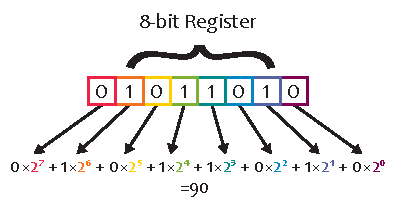
\includegraphics[width=0.75\linewidth]{Binary}
  \caption[Binary Coding]
  {We can encode information in a register in many ways. One encoding for positive numbers is to use a base-2
  positional system, like above, where the binary register \texttt{01011010} is mapped to the number 90.}
  \label{fig:binary}
\end{figure}

A \textbf{qubit} is similar to a bit in that it has two states, $\ket{0}$ and $\ket{1}$, except unlike a bit, it is specified
by a 2-dimensional vector, and evolves according to the rules of quantum mechanics. Due to the uniquely quantum
mechanical property of \emph{superposition}, we can no longer write the state of a single qubit (which we will
denote $\psi$) as either $\ket{0}$ or $\ket{1}$. Instead, we must write a down the vector sum of the two states,
which we define as follows:
\begin{align}
  \label{eqn:basisstates}
  \ket{0} = \svec{1\\0} && \ket{1} = \svec{0\\1}
\end{align}
\begin{equation}
  \ket{\psi} = \alpha \ket{0} + \beta \ket{1}
\end{equation}
where $\alpha$ and $\beta$ are complex numbers. If we were to take a measurement of this quantum state,
rather than getting back the value of this vector sum, we would measure the $\ket{0}$ state with probability
$|\alpha|^2$ and the $\ket{1}$ state with probability $|\beta|^2$. Since probabilities must sum to one, we also
get a normalization condition: $|\alpha|^2 + |\beta|^2 = 1$. The quantities $\alpha$ and $\beta$ are called
probability amplitudes, and they can take both positive and negative complex values
\footnote{Interestingly, the "complex" part of that state is unnessecary to get the extra computing power
  of a quantum computer\cite{doi:10.1142/S0219749913500019}. There's good reason that quantum mechanics 
  uses complex probability amplitudes\cite{2004quant.ph..1062A}, but if they were real, it turns out
  we can still do computations in \textsc{BQP} efficiently.} 
as long as their squared magnitudes sum to one. This gives us the first hint as to why quantum computing
might give us more power than a classical computer: their states can interact in a manner which mirrors
interference!

\begin{figure}
  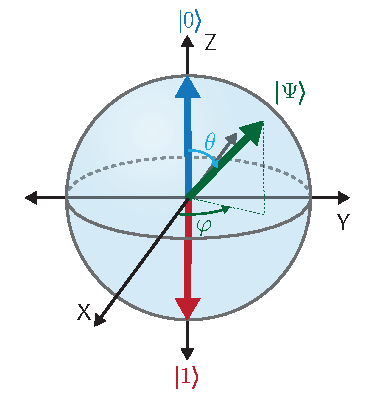
\includegraphics[width=0.5\linewidth]{BlochSphere}
  \caption[The Bloch Sphere representation of a qubit]
  {The state of a qubit can be represented as vector on the surface of a unit sphere. In this description, 
  the state is described by two angles: $\theta$ and $\psi$.}
  \label{fig:bloch}
\end{figure}

Too see how this is true, it's helpful to rewrite the above state in spherical coordinates. First, let's
write $\alpha = r_0e^{-i\varphi_1}$ and $\beta = r_1e^{-i\varphi_2}$. The normalization condition is now
$r_0^2 + r_1^2 = 1$, from which we can make the replacement $r_0 = \cos(\theta/2)$ and $r_1 = \sin(\theta/2)$.
We can also factor out the phase $\varphi_1$ to give:
\begin{equation}
\ket{\psi} = e^{-i\varphi_1}\left(
    \cos\left(\frac{\theta}{2}\right)\ket{0} + e^{-i(\varphi_2 - \varphi_1)}\sin\left(\frac{\theta}{2}\right)\ket{1}
  \right)
\end{equation}
The term $e^{-i\varphi_1}$ is called a global phase factor, and is equivalent to a multiplication by a unit vector,
which it's easy to see makes no difference to the probabilities of any measurement (a fact that will continue to be 
true even when we add more qubits). Another way of saying this is that the important information is encoded in 
the relative phase between the two states. So, let's make the replacement $\phi = \varphi_2 - \varphi_1$ and ignore
the global phase factor, which gives us the state:
\begin{equation}
  \ket{\psi} = \cos\left(\frac{\theta}{2}\right)\ket{0} + e^{-i\phi}\sin\left(\frac{\theta}{2}\right)\ket{1}
\end{equation}
This representation is shown visially in figure~\ref{fig:bloch} and is called the Bloch sphere representation
of a qubit.

Given this description, we can now start to think about what operations on a single qubit might look like.
While on a single bit, the only non-trivial operation we can perform is a flip ($0 \leftarrow 1$ and $1 \leftarrow 0$),
on a qubit we have whole host of operations that we can perform. The only limits we put on ourselves is that these operations
must leave us on the surface of the bloch sphere. In other words, after applying an operation, we must still
have a normalized state. From the Bloch representation, you may have already guessed that this means we
can only perform rotations... 

Switching back to the 2D vector representation of a qubit, then it's also clear that these operations
must correspond to $2\times2$ matrices. The act of performing an operation corresponds to multiplying
the qubit state by one of these matrices. In order to ensure that the length of the qubit vector $\ket{\psi}$
remains 1 at all times, the matrices we can use on our qubit must be unitary. That is, given the matrix $\boldsymbol{M}$,
its complex conjugate transpose $\boldsymbol{M}^\dagger = (\boldsymbol{M^{*}})^\mathrm{T}$ times itself is equal to 
the identity matrix: $\boldsymbol{M}^\dagger\boldsymbol{M} = \boldsymbol{I}$.

Let's define three unit rotation matrices as $\pi$ rotations around the $X, Y, Z$ axes. These have the symbols 
$\sigma_X, \sigma_Y, \sigma_Z$ respectively, and are called the Pauli matrices.
They have the values:
\begin{align}
  \sigma_X = \svec{0&1\\1&0} && \sigma_Y = \svec{0&-i\\i&0} && \sigma_Z = \svec{1&0\\0&-1}
\end{align}

We can build up arbitrary rotations from these unit vectors by taking various powers of these vectors
and multiplying them together. For example to apply a $\pi/2$ rotation around the y-axis to state $\ket{\psi}$
we would perform $\sqrt{\sigma_Y}\ket{\psi}$. A $2\pi$ rotation around the x-axis would be $\sigma_X\sigma_X\ket{\psi}$.

For example, starting from the $\ket{0}$ state, we might
perform a $\pi/2$ rotation around the y-axis, which, looking at the bloch sphere representation, ends up 
bringing the qubit down to the following state, which we will call $\ket{+}$:
\begin{equation}
  \ket{\psi} = \cos\left(\frac{\pi}{4}\right)\ket{0} + e^{0 i}\sin\left(\frac{\pi}{4}\right)\ket{1}
             = \frac{\ket{0} + \ket{1}}{\sqrt{2}} = \ket{+}
\end{equation}

We can also perform a rot


\section{Making Qubits in Semiconductors}
\label{sec:qcinsm}
  \subsection{The 2 Dimensional Electron Gas}
  \subsubsection{The Quantum Hall Effect}
  \subsubsection{Spin Orbit Interaction}
  \subsection{Quantum Dots}
  \subsection{Majorana Zero Modes}

\section{Architecture of a Quantum Computer}
\label{sec:arch}
  \subsection{Control Plane}
  \subsection{Readout}